\section{Data Preprocessing}
\label{sec:dataPreprocessing}

It is possible to preprocess the discriminating input variables or the training events prior 
to presenting them to a multivariate method. Preprocessing can be useful to reduce correlations 
among the variables, to transform their shapes into more appropriate forms, or to accelerate 
the response time of a method (event sorting). 

The preprocessing is completely transparent to 
the MVA methods. Any preprocessing performed for the training is automatically performed in 
the application through the Reader class. All the required information is stored in the 
weight files of the MVA method. The preprocessing methods normalisation and principal component 
decomposition are available for input and target variables, gaussianization, uniformization and decorrelation 
discussed below can only be used for input variables. 

Apart from five variable transformation methods mentioned above, an unsupervised variable selection method Variance Threshold is also implemented in TMVA. It follows a completely different processing pipeline. It is discussed in detail in section \ref{sec:varianceThreshold}. 

\subsection{Transforming input variables}
\label{sec:variableTransform}

Currently five preprocessing\index{Discriminating variables!preprocessing of}  
transformations\index{Discriminating variables!transformation of}
are implemented in TMVA:
\begin{itemize}
\item variable normalisation;
\item decorrelation via the square-root of the covariance matrix ;
\item decorrelation via a principal component decomposition;
\item transformation of the variables into Uniform distributions (``Uniformization'').
\item transformation of the variables into Gaussian distributions (``Gaussianisation'').
\end{itemize}
Normalisation and principal component decomposition can be applied to input and target variables, 
the other transformations can only be used for the input variables.  The transformations be performed for all input variables of for a selected subset of the input variables only. The latter is especially useful in situations where only some variables are correlated or the correlations are very different for different subsets.

All transformations can be performed separately for signal and background events
because their correlation patterns are usually different.\footnote
{
   Different transformations for signal and background events are only 
   useful for methods that explicitly distinguish signal and background 
   hypotheses. This is the case for the likelihood and PDE-RS classifiers.
   For all other methods the user must choose which transformation to use.
}

Technically, any transformation of the input and target variables is performed ``on the fly'' 
when the event is requested from the central \code{DataSet} class. The preprocessing 
is hence fully transparent to the MVA methods. Any preprocessing performed for the 
training is automatically also performed in the application through the Reader class. 
All the required information is stored in the weight files of the MVA method.
Each MVA method carries a variable
transformation type together with a pointer to the object of its
transformation class which is owned by the \code{DataSet}. If no
preprocessing is requested, an identity transform is applied. The
\code{DataSet} registers the requested transformations and takes care
not to recreate an identical transformation object (if requested)
during the training phase. Hence if two MVA methods wish to apply the
same transformation, a single object is shared between them. Each
method writes {\em its} transformation into its weight file once
the training has converged. For testing and application of an
MVA method, the transformation is read from the weight file and a
corresponding transformation object is created. Here each method
owns its transformation so that no sharing of potentially different
transformation objects occurs (they may have been obtained with
different training data and/or under different conditions). A
schematic view of the variable transformation interface used in TMVA
is drawn in Fig.~\ref{fig:VariableTransform}.
\begin{figure}[t]
  \begin{center}
	  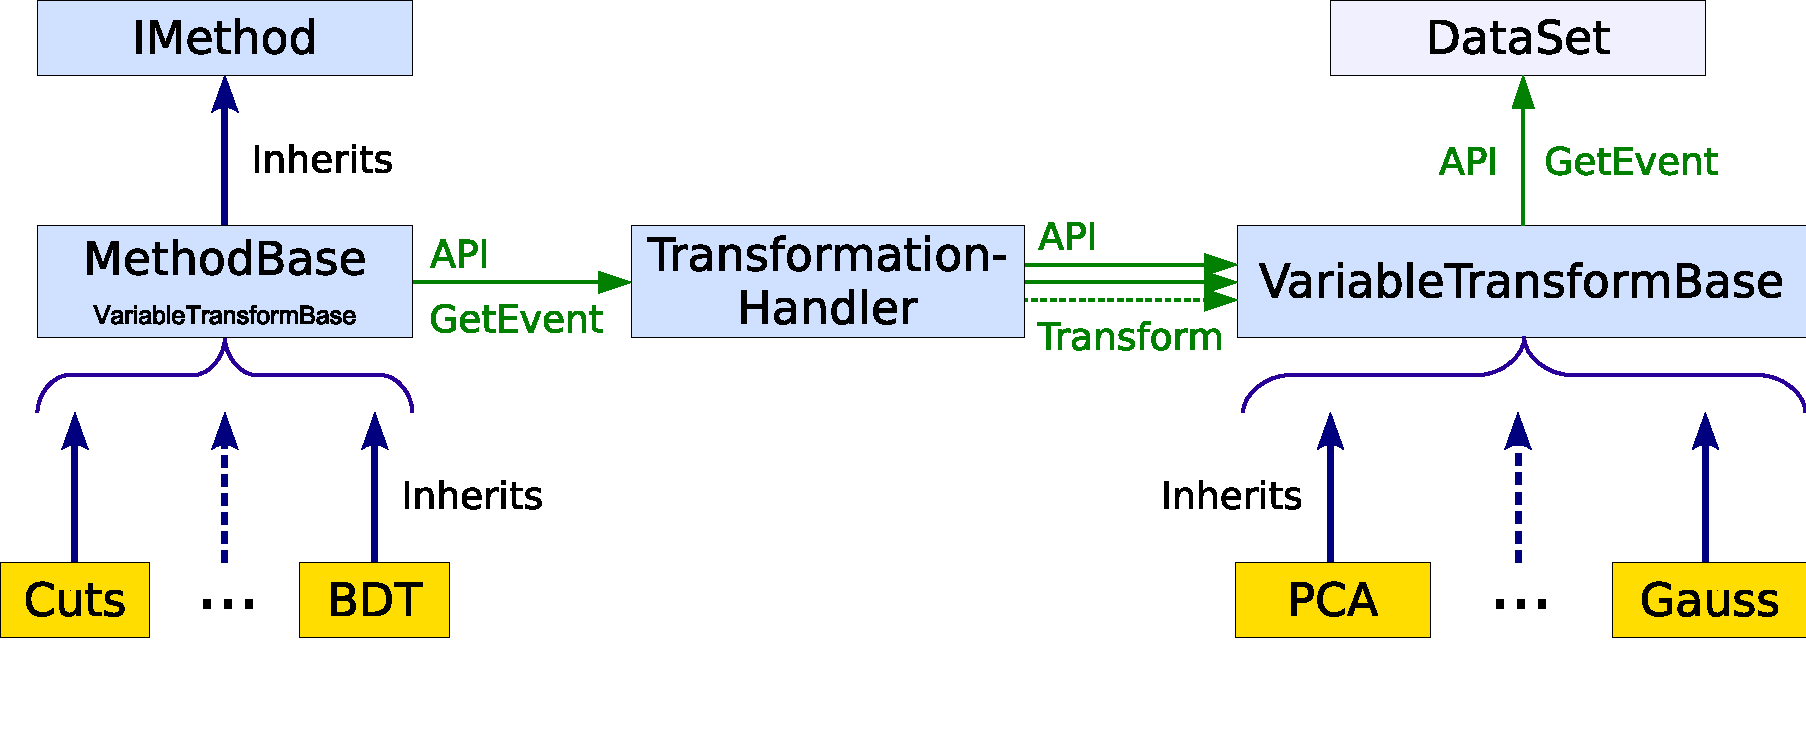
\includegraphics[width=0.90\textwidth]{plots/VariableTransforms}
  \end{center}
  \vspace{-1.1cm}
  \caption[.]{Schematic view of the variable transformation interface implemented in 
    TMVA. Each concrete MVA method derives from \code{MethodBase} 
    (interfaced by \code{IMethod}), which holds a protected member object 
    of type \code{TransformationHandler}. In this object a list of objects 
    derived from \code{VariableTransformBase} which are the implementations of 
    the particular variable transformations available in TMVA is stored. 
    The construction of the concrete 
    variable transformation objects proceeds in \code{MethodBase} according 
    to the transformation methods requested in the option string. The events
    used by the MVA methods for training, testing and final classification (or regression)
    analysis are read via an API of the \code{TransformationHandler} class, 
    which itself reads the events from the \code{DataSet} and applies 
    subsequently all initialised transformations. The \code{DataSet} 
    fills the current values into the reserved event 
    addresses (the event content may either stem from the training or 
    testing trees, or is set by the user application via the \code{Reader} 
    for the final classification/regression analysis). The \code{TransformationHandler}
    class ensures the proper transformation of all events seen by 
    the MVA methods.
}
\label{fig:VariableTransform}
\end{figure}

\subsubsection{Variable normalisation\index{Discriminating variables!normalisation of}}
\label{sec:normalisation}

Minimum and maximum values for the variables to be transformed are determined from the training 
events and used to linearly scale these input variables to lie within $[-1,1]$. 
Such a transformation is useful to allow direct comparisons between the MVA weights 
assigned to the variables, where large absolute weights may indicate strong separation power. 
Normalisation may also render minimisation processes, such as the adjustment of 
neural network weights, more effective. 

\subsubsection{Variable decorrelation\index{Discriminating variables!decorrelation of}}
\label{sec:decorrelation}

A drawback of, for example, the projective likelihood classifier (see 
Sec.~\ref{sec:likelihood}) is that it ignores correlations among the discriminating 
input variables. Because in most realistic use cases this is not an accurate 
conjecture it leads to performance loss. Also other classifiers, such as rectangular 
cuts or decision trees, and even multidimensional likelihood approaches underperform
in presence of variable correlations.

Linear correlations, measured in the training sample, can be taken into account 
in a straightforward manner through computing the square-root of the covariance 
matrix. The square-root of a matrix $C$ is the matrix $C^\prime$ that multiplied 
with itself yields $C$: $C=(C^\prime)^2$. TMVA computes the square-root matrix 
by means of diagonalising the (symmetric) covariance matrix
\beq
    D=S^T C S \hspace{0.5cm}\Rightarrow \hspace{0.5cm}
    C^\prime=S\sqrt{D}S^T\,,
\eeq
where $D$ is a diagonal matrix, and where the matrix $S$ is symmetric. The linear 
decorrelation of the selected variables is then obtained by multiplying the 
initial variable tuple ${\bf x}$ by the inverse of the square-root matrix
\beq
      {\bf x} \mapsto (C^\prime)^{-1}{\bf x}\:.
\eeq


The decorrelation is complete only for linearly correlated and Gaussian distributed 
variables. In situations where these requirements are not fulfilled
only little additional information can be recovered by the decorrelation
procedure. For highly nonlinear problems the performance may even become
worse with linear decorrelation. Nonlinear methods without prior variable 
decorrelation should be used in such cases.





\subsubsection{Principal component decomposition\index{Discriminating variables!PCA of}}
\label{sec:pca}

Principal component decomposition\index{Principal component decomposition, analysis}
or principal component analysis (PCA) as presently applied in TMVA is not very
different from the above linear decorrelation. In common words, PCA is a linear 
transformation that rotates a sample of data points such that the maximum 
variability is visible. It thus identifies the 
most important gradients. In the PCA-transformed coordinate system, the 
largest variance by any projection of the data comes to lie on the first 
coordinate (denoted the {\em first principal component}), the second 
largest variance on the second coordinate, and so on. PCA can thus be used
to reduce the dimensionality of a problem (initially given by the number of 
input variables) by removing dimensions with insignificant variance. This 
corresponds to keeping lower-order principal components and ignoring 
higher-order ones. This latter step however goes beyond straight variable 
transformation as performed in the preprocessing steps discussed here 
(it rather represents itself a full classification method). Hence all principal
components are retained here.

The tuples ${\bf x}_U^{\rm PC}(i)=(x_{U,1}^{\rm PC}(i),\dots,x_{U,\Nvar}^{\rm PC}(i))$ 
of principal components of a tuple of input variables ${\bf x}(i)=(x_1(i),\dots,x_{\Nvar}(i))$,
measured for the event $i$ for signal ($U=S$) and background ($U=B$),
are obtained by the transformation
\beq
\label{eq:pca}
   x_{U,k}^{\rm PC}(i) = \sum_{\ell=1}^{\Nvar}
                         \left(x_{U,\ell}(i) - \overline x_{U,\ell}\right)
                         v^{(k)}_{U,\ell}\,,
   \hspace{0.5cm}\forall k=1,\Nvar\,.
\eeq
The tuples $\overline{\bf x}_{U}$ and ${\bf v}_{U}^{(k)}$ are the sample 
means and eigenvectors, respectively. They are computed by the ROOT class 
\code{TPrincipal}. The matrix of eigenvectors 
$V_U=({\bf v}^{(1)}_{U}\!,\dots,{\bf v}^{(\Nvar)}_{U})$ 
obeys the relation
\beq
   C_U\cdot V_U = D_U\cdot V_U\,,
\eeq
where $C$ is the covariance matrix of the sample $U$, and $D_U$ is the tuple
of eigenvalues. As for the preprocessing described in 
Sec.~\ref{sec:decorrelation}, the transformation~(\ref{eq:pca}) eliminates
linear correlations for Gaussian variables.

\subsubsection{Uniform and Gaussian transformation of variables 
(``Uniformisation'' and ``Gaussianisation'')\index{Discriminating variables!Gaussianisation of} \index{Discriminating variables!Uniformisation of}}
\label{sec:gaussianisation}

The decorrelation methods described above require linearly correlated and Gaussian 
distributed input variables. In real-life HEP applications this is however rarely the 
case. One may hence transform the variables prior to their decorrelation such that their 
distributions become Gaussian. The corresponding transformation function is conveniently
separated into two steps: first, transform a variable into a uniform distribution
using its cumulative distribution function\footnote
{
   The cumulative distribution function $F(x)$ of the variable $x$ is given by 
   the integral $F(x)=\intl_{-\infty}^{x}\!\!\xPDF(x^\prime)\,d x^\prime$, where 
   $\xPDF$ is the probability density function of $x$.
} 
obtained from the training data (this transformation is identical to the probability integral transformation 
(``Rarity'') 
introduced in Sec.~\ref{sec:otherRepresentations} on page~\pageref{sec:otherRepresentations});
second, use the inverse error function to transform the uniform distribution into 
a Gaussian shape with zero mean and unity width. As for the
other transformations, one needs to choose which class of events (signal or background) is to be 
transformed and hence, for the input variables (Gaussianisation is not available 
for target values), it is only possible to transform signal {\em or} background into 
proper Gaussian distributions (except for classifiers testing explicitly both
hypotheses such as likelihood methods). Hence a discriminant input variable $x$ 
with the probability density function  $\xPDF$ is transformed as follows 
\beq
\label{eq:gaussianisation}
   x \mapsto \sqrt{2}\cdot {\rm erf}^{-1}\!\!
             \left( 2\cdot \!\!\intl_{-\infty}^{x}\!\!\xPDF(x^\prime)\,d x^\prime -1 \right)\:.
\eeq
A subsequent decorrelation of the transformed variable tuple sees Gaussian 
distributions, but most likely non-linear correlations as a consequence of the 
transformation~(\ref{eq:gaussianisation}). The distributions obtained after the 
decorrelation may thus not be Gaussian anymore. It has been suggested that 
iterating Gaussianisation and decorrelation more than once may improve the 
performance of likelihood methods (see next section).

\subsubsection{Booking and chaining transformations for some or all input variables}\index{Booking and chaining variable transformations}

Variable transformations to be applied prior to the MVA training (and application) 
can be defined independently for each MVA method with the booking option 
{\tt VarTransform=<type>}, where {\tt <type>} denotes the desired transformation 
(or chain of transformations). The available transformation types are normalisation, 
decorrelation, principal component analysis and Gaussianisation, which are labelled by 
\code{Norm}, \code{Deco}, \code{PCA}, \code{Uniform}, \code{Gauss}, respectively, or, equivalently, 
by the short-hand notations \code{N}, \code{D}, \code{P}, \code{U} , \code{G}.

Transformations can be {\em chained} allowing the consecutive application of all defined 
transformations to the variables for each event.
For example, the above Gaussianisation and decorrelation sequence would be programmed by 
\code{VarTransform=G,D}, or even \code{VarTransform=G,D,G,D} in case of two iterations 
(instead of the comma ``,'', a ``+'' can be equivalently used as chain operator, 
i.e. \code{VarTransform=G+D+G+D}). The ordering of the transformations goes from 
left (first) to right (last). 

\begin{codeexample}
\begin{tmvacode}
factory->BookMethod( TMVA::Types::kLD, "LD_GD", "H:!V:VarTransform=G,D");
\end{tmvacode}
\caption[.]{\codeexampleCaptionSize Booking of a linear discriminant
  (LD) classifier with Gaussianisation and decorrelation for all input
  variables.  }
\end{codeexample}

By default, the transformations are computed with the use of all training events. It is 
possible to specify the use of a specific class only (\eg, \code{Signal}, \code{Background}, 
\code{Regression}) by attaching {\tt \_<class name>} to the user option -- 
where {\tt <class name>} has to be replaced by the actual class name 
(\eg, \code{Signal}) -- which defines the transformation (\eg, {\tt VarTransform=G\_Signal}). 
A complex transformation option might hence look like {\tt VarTransform=D,G\_Signal,N}.
The attachment {\tt \_AllClasses} is equivalent to the default, where events from all 
classes are used.

\begin{codeexample}
\begin{tmvacode}
factory->BookMethod( TMVA::Types::kLD, "LD_GDSignal", "H:!V:VarTransform= \
G_Signal,D_Signal");
\end{tmvacode}
\caption[.]{\codeexampleCaptionSize Booking of a linear discriminant
  (LD) classifier where the Gaussianisation and decorrelation
  transformations are computed from the signal events only.  }
\end{codeexample}

By default, all input variables are transformed when booking a
transformation. In many situations however, it is desirable to apply a
transformation only to a subset of all variables\footnote{As
  decorrelation for example is only reasonable if the variables have
  strong ``linear'' correlations, it might be wise to apply the
  decorrelation only to those variables that have linear
  correlations}.  Such a selection can be achieved by specifying the
variable names separated by commas in brackets after the
transformation name,
i.e. \code{VarTransform=N(var2,var1,myvar3)}. Alternatively the
variables and targets can be denoted by their position
\code{_V<index>_} (for input variables) and \code{_T<index>_} (for
targets) where the index is the position of the variable (target)
according to the order in which the variables where defined to the
factory (e.g. \code{VarTransform=N(_V0_,_V3_,_T3_)}.  The numbering
starts with 0 and the ordering of the variables within the parentheses
has no impact.  To address all variables (targets) the keywords
\code{_V_} and \code{_T_} can be used.  The result of a transformation
is written back into the same variables. For instance in the case of
the principal component analysis transformation the first (and most
important) eigenvalue is written into the variable with the smallest
index, the second eigentvalue into the variable with the second lowest
index and so forth. Input variables and targets can only be
transformed at the same time if each variable is transformed
independently. This is the case for the normalisation transformation.

Transformations of variable subsets can also be chained. For example,
in \code{VarTransform=N+P(_V0_,var2,_V4_)+P(_T_)_Background+G_Signal},
first all variables and targets are normalized with respect to all
events, then the variables with the indices 0 and 4 and the variable
\code{var2} are PCA transformed, subsequently all targets are PCA
transformed with respect to the background events and finally all
variables are gaussianised with respect to the signal events.

\begin{codeexample}
\begin{tmvacode}
factory->BookMethod( TMVA::Types::kLD, "LD_DSubset", "H:!V:VarTransform= \
D(_V0_,var2)");
\end{tmvacode}
\caption[.]{\codeexampleCaptionSize Booking of a linear discriminant
  (LD) classifier where only the first variable and the variable
  labeled \code{var2} are subject to a decorrelation transformation.
}
\end{codeexample}

\subsection{Variable selection based on variance}
\label{sec:varianceThreshold}
In high energy physics and machine learning problems, we often encounter datasets which have large number of input variables. However to extract maximum information from the data, we need to select the relevant input variables for the multivariate classification and regression methods implemented in TMVA. Variance Threshold is a simple unsupervised variable selection method which automates this process.
It computes weighted variance $\sigma^2_{j}$ for each variable $j = 1,\dots,{\Nvar}$ and ignores the ones whose variance lie below a specific threshold. Weighted variance for each variable is defined as follows:
\beq
\label{eq:variancecalculation}
\sigma^2_{j} = \frac{\sum_{i=1}^N w_i (x_j(i) - \mu_{j})^2}{\sum_{i=1}^N w_i}
\eeq

where $N$ is the total number of events in a dataset, ${\bf x}(i)=(x_1(i),\dots,x_{\Nvar}(i))$ denotes each event $i$ and $w_i$ is the weight of each event. Weighted mean $\mu_{j}$ is defined as: 

\beq
\label{eq:meanecalculation}
\mu_j = \frac{\sum_{i=1}^N w_i x_{j}(i)}{\sum_{i=1}^N w_i}
\eeq
Unlike above five variable transformation method, this Variance Threshold method is implemented in DataLoader class. After loading dataset in the DataLoader object, we can apply this method. It returns a new DataLoader with the selected variables which have variance strictly greater than the threshold value passed by user. Default value of threshold is zero i.e. remove the variables which have same value in all the events. 

\begin{codeexample}
\begin{tmvacode}
// Threshold value of variance = 2.95
TMVA::DataLoader* transformed_loader1 = loader->VarTransform("VT(2.95)");
// No threshold value passed in below example, hence default value = 0
TMVA::DataLoader* transformed_loader2 = loader->VarTransform("VT");
\end{tmvacode}
\caption[.]{\codeexampleCaptionSize \code{VT} stands for Variance Threshold. Parameter passed to \code{VarTransform} method is just a single string. String strictly follows either of the above two formats for Variance Threshold otherwise method would raise an error. 
}
\end{codeexample}


\subsection{Binary search trees\index{Binary search trees}} 
\label{sec:binaryTrees}

When frequent iterations over the training sample need to be performed, it is helpful 
to sort the sample before using it. Event sorting in {\em binary trees} is employed 
by the MVA methods rectangular cut optimisation\index{Cut optimisation},  
PDE-RS\index{PDE-RS} and k-NN\index{kd-tree}. While the former two classifiers rely on 
the simplest possible binary tree implementation, k-NN uses on a better performing 
{\em kd-tree} (\cf\  Ref.~\cite{kd-tree}).\index{kd-tree}

Efficiently searching for and counting events that lie inside a multidimensional
volume spanned by the discriminating input variables is accomplished with the use of a 
binary tree search algorithm~\cite{BinaryTree}.\footnote
{
   The following is extracted from Ref.~\cite{CarliKoblitz} for a two-dimensional 
   range search example.
   Consider a random sequence of signal events $e_i(x_1, x_2)$, $i = 1,2,\dots$, 
   which are to be stored in a binary tree. The first event in the sequence 
   becomes by definition the topmost node of the tree. The second event 
   $e_2(x_1, x_2)$ shall have a larger $x_1$-coordinate than the first event, 
   therefore a new node is created for it and the node is attached to the first
   node as the right child (if the $x_1$-coordinate had been smaller, the 
   node would have become the left child). Event $e_3$ shall have a larger 
   $x_1$-coordinate than event $e_1$, it therefore should be attached to 
   the right branch below $e_1$. Since $e_2$ is already placed at that 
   position, now the $x_2$-coordinates of $e_2$ and $e_3$ are compared, and,
   since $e_3$ has a larger $x_2$, $e_3$ becomes the right child of the node 
   with event $e_2$.
   The tree is sequentially filled by taking every event and, while 
   descending the tree, comparing its $x_1$ and $x_2$ coordinates with 
   the events already in place. Whether $x_1$ or $x_2$ are used for the 
   comparison depends on the level within the tree. On the first level, 
   $x_1$ is used, on the second level $x_2$, on the third again $x_1$ 
   and so on.
}
It is realised in the class \code{BinarySearchTree}, which 
inherits from \code{BinaryTree}, and which is also employed to grow decision 
trees (\cf\  Sec.~\ref{sec:bdt}). The amount of computing time needed to 
sort $N$ events into the tree is~\cite{CarliKoblitz} 
$\propto\sum_{i=1}^N\ln_2(i)=\ln_2(N!)\simeq N\ln_2N$. 
Finding the events within the tree which lie in a given volume is done 
by comparing the bounds of the volume with the coordinates of the events 
in the tree. Searching the tree once requires a CPU time that is
$\propto\ln_2N$, compared to $\propto N^\Nvar$ without prior event sorting.

